\documentclass[11pt]{article}

\usepackage[margin=1in]{geometry}
\usepackage{amsmath,amsthm}
\usepackage{mathtools}
\usepackage{graphicx}
\usepackage{dsfont}  % \mathds{1} indicator (OldStandard-Math lacks a bold digit 1)
% Old-style journal look (after tex.stackexchange.com/q/645339): OldStandard text + matching
% OpenType math, small-caps headings, run-in paragraphs. Requires lualatex (pinned in .latexmkrc).
\usepackage{OldStandard}
\usepackage{unicode-math}
\setmathfont{OldStandard-Math.otf}
\usepackage{titlesec}
\usepackage{fancyvrb}
\usepackage[hidelinks]{hyperref}

\linespread{1.15}
\setlength{\parindent}{2em}
\titleformat{\section}{\normalfont\large\scshape\bfseries}{\thesection.}{0.6em}{}
\titleformat{\subsection}{\normalfont\scshape\bfseries}{\thesubsection.}{0.5em}{}
\titleformat{\paragraph}[runin]{\bfseries\scshape}{}{0pt}{}[.]
\titlespacing*{\paragraph}{\parindent}{0.4em}{0.6em}

\newtheoremstyle{oldplain}{}{}{\itshape}{}{\scshape}{.}{.5em}{}
\newtheoremstyle{oldrem}{}{}{\normalfont}{}{\scshape}{.}{.5em}{}
\theoremstyle{oldplain}
\newtheorem{proposition}{Proposition}
\theoremstyle{oldrem}
\newtheorem{definition}{Definition}
\newtheorem{remark}{Remark}

\DeclareMathOperator{\Poisson}{Poisson}
\newcommand{\Pzero}{P_{0}}
\newcommand{\ball}[2]{B_{#1}(#2)}
\newcommand{\E}{\mathbb{E}}
\newcommand{\Prob}{\mathbb{P}}

\title{\scshape Scoring, substitution matrices and score aggregation for
TCR antigen-specificity search}
\author{The vdjmatch authors\thanks{Supplementary technical note for the \texttt{vdjmatch} software;
intended as supplementary material to the main manuscript.}}
\date{\small\textit{vdjmatch technical appendix} --- draft, regenerated from
\texttt{bench/gen\_vdjam.py}, \texttt{bench/loo\_vdjam.py}, \texttt{bench/gen\_appendix\_assets.py}}

\begin{document}
\maketitle

\begin{abstract}
\noindent
\texttt{vdjmatch} annotates T-cell receptor (TCR) clonotypes by antigen specificity through fuzzy
CDR3 search against a labelled database (VDJdb), built on the \texttt{seqtree} search core. This note
documents the \emph{scoring} layer: how CDR3 similarity is scored, the data-driven TCR substitution
matrix (VDJAM) and why it is region-structured, and how per-hit scores are aggregated into a
control-calibrated significance. CDR3 loops resist the assumptions behind BLOSUM/PAM --- they cannot
be multiply aligned across clonotypes of different length, and germline-encoded flanks
(\texttt{CASS}\dots) are so over-conserved that a naive matrix conflates germline bias with selection.
We give a position-debiased log-odds estimator that isolates the substitution signal, show
empirically that this signal lives in the non-template (NDN) core while the V/J flanks are
germline-determined, and demonstrate the consequences on worked examples (GIL, NLV) using the
alignments and CIGAR strings produced by \texttt{seqtree}. The E-value theory used for significance is
derived in the companion \texttt{seqtree} appendix; here we summarize it and give the paired-chain
extension.
\end{abstract}

\section{The search-and-score framework}
Given a query CDR3 $q$ and a labelled reference set $D$ (VDJdb), \texttt{vdjmatch} retrieves the
neighbours of $q$ within a fixed scope $\theta=(s,i,d,t)$ (max substitutions, insertions, deletions,
total edits) using the \texttt{seqtree} engine, which defines a ball $\ball{\theta}{q}=\{x:
\mathrm{edit}(q,x)\le\theta\}$ and returns, per hit, the edit decomposition and a matrix-weighted
alignment. The matrix enters as a \emph{ranking} score inside the ball; the ball itself (an edit
budget) bounds the candidate set. Each hit carries its antigen labels, an extended CIGAR
($=$/$\mathtt{X}$/$\mathtt{I}$/$\mathtt{D}$), and an alignment score. Significance comes from comparing
the neighbour count to a matched background control (\S\ref{sec:agg}).

\section{Substitution scoring and the VDJAM matrix}\label{sec:vdjam}

\paragraph{How BLOSUM is built, and why it does not transfer.} BLOSUM is a log-odds matrix estimated
from the BLOCKS database of \emph{ungapped multiple-alignment blocks} of conserved protein regions. Its
recipe is: (i) take many trusted blocks --- columns of homologous, gaplessly aligned residues; (ii)
cluster sequences within a block above a percent-identity threshold and down-weight within-cluster pairs
so abundant near-duplicates do not dominate; (iii) count, over all blocks, how often residues $a$ and
$b$ co-occur in the \emph{same alignment column}, $q_{ab}$; (iv) score
$s(a,b)=\tfrac1\lambda\log\!\big(q_{ab}/p_ap_b\big)$ against the \emph{global} background frequencies
$p_a$. The signal is ``which residues substitute for one another within conserved, column-homologous
positions,'' and the background is position-independent.

CDR3 loops break every step. (i) There is no trusted multiple alignment: same-specificity CDR3s differ
in length and have no column homology, so ``alignment columns'' do not exist. (ii) The germline-encoded
ends are over-conserved --- essentially every human TRB CDR3 begins \texttt{CASS} and ends in a short J
motif --- so a \emph{global} background $p_a$ is wrong: an alanine in the N-terminal \texttt{CASS} is
germline-fixed and carries no specificity signal, while an alanine in the centre does, yet BLOSUM would
score them identically. A single global matrix estimated over all positions thus conflates germline
conservation with antigen-driven selection.

\paragraph{What VDJAM changes (point by point).} VDJAM keeps the log-odds idea but replaces the two
broken ingredients. (a) \emph{Observation unit}: instead of columns of a multiple alignment, the unit is
a \emph{same-antigen single-substitution pair} --- two CDR3s annotated to the same epitope, equal length,
differing at exactly one position; this is the only ``aligned residue pair'' obtainable without a
multiple alignment, and (like a BLOCKS column pair) it records two residues that are interchangeable
without changing function (here, specificity). (b) \emph{Background}: instead of a global $p_a$, a
\emph{position-specific} background $\mathrm{bg}(\cdot\mid L,p)$ (the residue frequency at that length and
position) is used, so over-conserved columns are normalized away analytically rather than masked by hand.
(c) \emph{Redundancy}: BLOSUM's percent-identity clustering is replaced --- partly by the position-specific
background (germline-shared residues are ``expected'' and contribute little), and prospectively by the
control-calibrated significance layer (\S\ref{sec:agg}) that already discounts convergent public clones;
per-clonotype clustering can be added exactly as in BLOSUM if needed. (d) \emph{Scope}: BLOSUM is one
global matrix; VDJAM is estimated per chain and per region, because (next paragraph) only the NDN core
carries a transferable substitution signal.

\paragraph{Observation unit and estimator.} We replace ``alignment columns'' with \emph{same-antigen
single-substitution pairs}: ordered pairs of CDR3s annotated to the same epitope, of equal length,
differing at exactly one position --- the only clean substitution signal extractable without a
multiple alignment. For a substitution $a\!\leftrightarrow\! b$ observed at position $p$ in a CDR3 of
length $L$ on chain $c$, let $\mathrm{bg}(\cdot\mid L,p)$ be the residue frequency at position $p$
among all length-$L$ chain-$c$ CDR3s. With $f(a,b)$ the observed count of $\{a,b\}$ events and
\begin{equation}\label{eq:vdjam}
  e(a,b)=\!\!\sum_{\text{event slots }(L,p)}\!\! n_{L,p}\,\big[\mathrm{bg}(a\mid L,p)\,\mathrm{bg}(b\mid L,p)
  + \mathrm{bg}(b\mid L,p)\,\mathrm{bg}(a\mid L,p)\big],\qquad
  \mathrm{VDJAM}(a,b)=\log_2\frac{f(a,b)+\alpha}{e(a,b)+\alpha},
\end{equation}
where $n_{L,p}$ is the number of observed events at $(L,p)$ and $\alpha$ a Laplace pseudocount. The
key point is that the background is \emph{position-specific}: at an over-conserved column the residue
frequency is peaked, so substitutions there are both rare (small $f$) and ``expected'' (matched $e$),
and contribute $\approx0$ to the log-odds --- the germline bias is removed analytically rather than by
hand-masking. The matrix is consumed by \texttt{seqtree} via the squared-distance penalty
$\mathrm{pen}(a,b)=s_{aa}+s_{bb}-2s_{ab}$ (\texttt{SubstitutionMatrix.from\_similarity}); a dominant
uniform diagonal makes higher learned similarity rank a substitution better.

\paragraph{Region structure: NDN is learned, V/J are germline-determined.} A CDR3 is V-germline prefix
$\,\cdot\,$ NDN insert $\,\cdot\,$ J-germline suffix. Estimating \eqref{eq:vdjam} separately by region
shows (Fig.~\ref{fig:region}) that the substitution signal --- the agreement with general amino-acid
chemistry, measured as correlation with BLOSUM62 --- is concentrated in the NDN core (TRB
$r\!=\!0.42$, TRA $0.35$), whereas the V flank carries almost none (TRB $0.08$, TRA $0.07$): V-flank
``substitutions'' are dominated by germline allele differences, not free chemistry. This motivates a
two-part model: \textbf{VDJAM is learned for the NDN core}, while the \textbf{V and J flanks are
auto-computed} from the germline V/J sequences and their trimming. Concretely, a CDR3 position derived
from V- (or J-) germline is near-invariant when it survives trimming and reverts to the random-insert
background when trimmed; so the V/J contribution is a per-position conservation profile $w(p)=\Pr[\text{position
}p\text{ is germline-retained}]$, determined by the gene's trimming-length distribution, rather than a
substitution matrix learned from data. Combined, the NDN matrix scores the core and $w(p)$ down-weights
substitutions at germline-retained flanks (realized through a per-position weighting of the base
matrix). \emph{Status:} the NDN matrix and the region decomposition are implemented and evaluated
below; the germline$+$trimming V/J profile (from the OLGA recombination model, via \texttt{mirpy}) is
in progress.

\begin{figure}[ht]\centering
  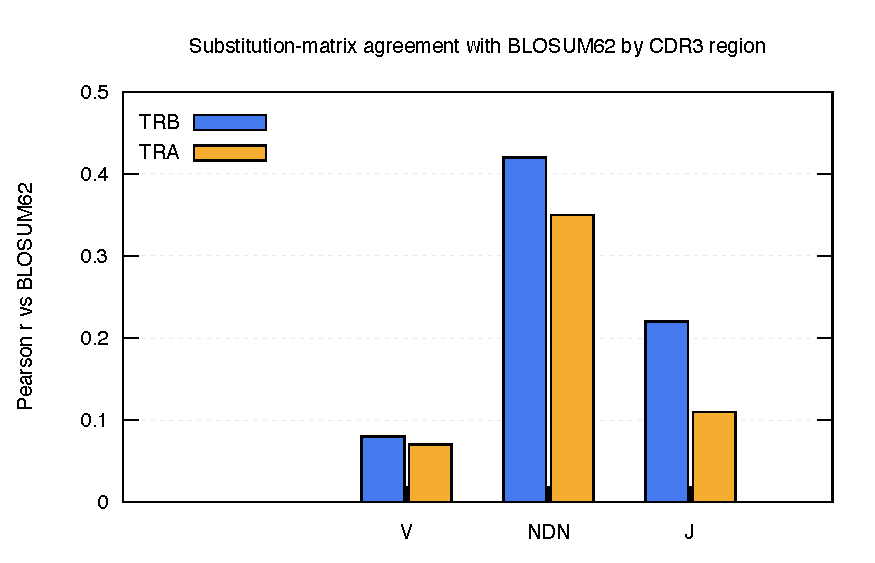
\includegraphics[width=0.62\linewidth]{figures/region_corr.pdf}
  \caption{Per-region agreement of the learned CDR3 substitution matrix with BLOSUM62 (Pearson $r$ of
  off-diagonal scores), human VDJdb. The free-substitution signal lives in the NDN core; the V flank is
  germline-determined.}
  \label{fig:region}
\end{figure}

\section{Score aggregation and significance}\label{sec:agg}
\paragraph{Per-hit to per-query.} A region-aware similarity score sums the NDN matrix score over the
core and the (down-weighted) flank contributions; this is available as an optional ranking score and
generalizes the legacy cloglog generalized-linear aggregation over V/CDR1/CDR2/J/CDR3.

\paragraph{Control-calibrated E-value (primary).} Immune repertoires are biologically redundant, so an
i.i.d.\ null over-calls. \texttt{vdjmatch} instead counts a query's VDJdb neighbours within the ball
and compares to the count expected from a matched background control: with $N=|D|$, $M$ the control
size and $n_C$ the control neighbour count, $\E=(N/M)\,n_C$ is the expected number of VDJdb neighbours
by chance and $p_{\mathrm{enrich}}=\Prob(\Poisson(\E)\ge n_{D})$ is the enrichment significance ---
significant only when a clonotype has \emph{more} VDJdb neighbours than the generative background
predicts. The Poisson/Chen--Stein theory, the punctured (self-excluding) null and the choice of $M$ are
derived in the companion \texttt{seqtree} appendix.

\paragraph{Paired $\alpha\beta$ E-value.} The null factorization is not an approximation of
convenience: $\alpha$ and $\beta$ chains pair \emph{almost without constraint} in the repertoire at
large, as shown by integrating structural and paired-sequencing data~\cite{Shcherbinin2020}, so under
the background (generative) law the joint ball mass genuinely factorizes,
$\pi_0^{\alpha\beta}\approx\pi_0^\alpha\pi_0^\beta$. Crucially, the \emph{same} analysis finds that
\emph{antigen-driven selection distorts} this uniform pairing landscape --- i.e.\ conditioned on an
epitope the two chains are \emph{not} independent. This is exactly the structure the joint E-value
exploits: the null factorizes (background pairing is unconstrained), so among the $N$ paired VDJdb
complexes the expected number of chance joint matches is $\E_{\alpha\beta}=N\,\pi_0^\alpha\pi_0^\beta$
with $p$ the Poisson tail on the count of complexes matched in \emph{both} chains; an excess over this
factorized null is precisely the epitope-conditional dependence (co-selection of $\alpha$ and $\beta$)
that signals a true specificity. Because the joint null is far smaller than either chain's, true pairs
are dramatically more significant: on the paired TCRvdb benchmark, $296/300$ pairs match a complex and
$295/296$ ($99.7\%$) recover the correct epitope, with joint $p$ down to $3.6\times10^{-9}$. (When the
two chains' hits are treated as independent tests, the equivalent statistic is Fisher's combination of
the per-chain enrichments; the appendix \texttt{seqtree} co-occupancy term quantifies the residual
dependence.)

\section{Results: does VDJAM help?}
A matrix derived from same-antigen pairs must be tested on epitopes it never saw, or the evaluation is
circular. For each held-out epitope $E^\ast$ we re-derive the NDN matrix from \emph{all other}
epitopes, then run VDJdb-vs-VDJdb retrieval on $E^\ast$ (exact self excluded), ranking neighbours by
each matrix, and score the micro precision--recall AUC for ``neighbour shares $E^\ast$''. Across the
eight largest TRB epitopes (scope $2$, Fig.~\ref{fig:loo}) the learned NDN matrix improves over unit
(edit-distance) cost (mean $\Delta\mathrm{PR\text{-}AUC}=+0.018$) and is on par with BLOSUM62
($-0.009$; better on $4/8$). At this scope the search ball already supplies most of the
specific-vs-nonspecific discrimination and the matrix only re-ranks within it; the larger gains are
expected from the region-aware combination (NDN matrix $+$ germline/trimming flank weighting) and at
wider scopes, which is the current line of work.

\begin{figure}[ht]\centering
  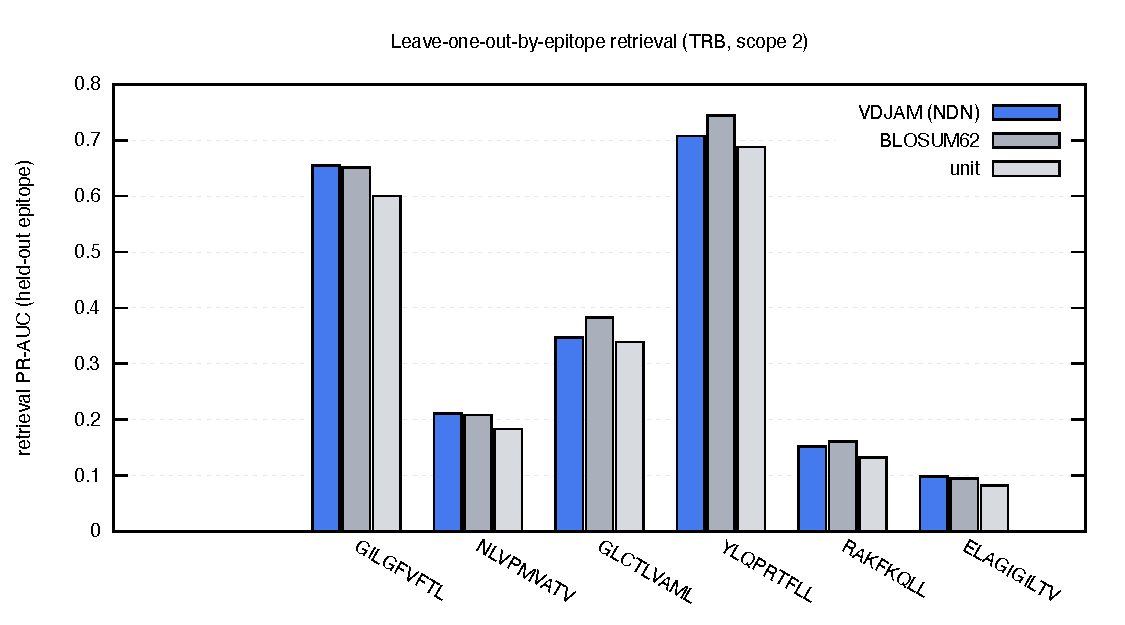
\includegraphics[width=0.78\linewidth]{figures/loo_prauc.pdf}
  \caption{Leave-one-out-by-epitope retrieval PR-AUC (TRB, scope $2$): the NDN VDJAM matrix versus
  BLOSUM62 and unit cost on epitopes excluded from matrix estimation.}
  \label{fig:loo}
\end{figure}

\section{Worked examples}
\paragraph{Pairwise (different lengths).} \texttt{seqtree} aligns CDR3s of differing length, placing
indels where the loop genuinely lengthens. The edit-distance alignments below (influenza GIL-specific
TRB CDR3s) show the conserved \texttt{CASS} V-anchor and \texttt{DTQYF} J-motif with substitutions and
indels confined to the central NDN core:
{\small\VerbatimInput{aln/pairwise.txt}}

\paragraph{Multiple (same length).} Aligning same-length same-epitope CDR3s (no indels needed) makes
the conservation profile explicit (Figs.~\ref{fig:gil}--\ref{fig:nlv}): columns are shaded by
conservation, dark at the germline-determined \texttt{CASS} prefix and J motif, light through the
variable NDN core. This is the structural counterpart of the finding of
Shcherbinin~et~al.~\cite{Shcherbinin2023} that specificity-preserving CDR3 substitutions occur
predominantly outside the peptide/MHC-contacting positions while preserving the loop backbone --- i.e.\
the tolerated variation we score in the NDN core is exactly the variation that does not break
recognition.

\begin{figure}[ht]\centering
  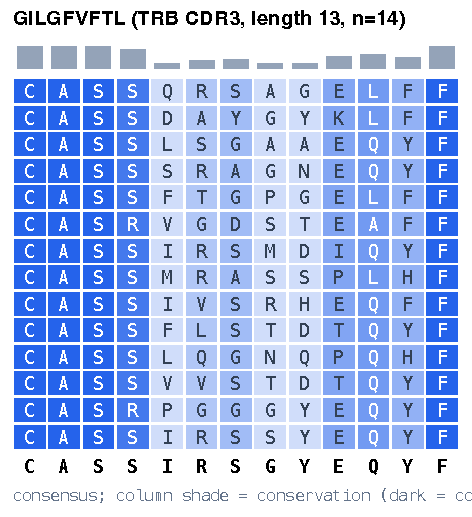
\includegraphics[width=0.66\linewidth]{aln/GILGFVFTL_msa.pdf}
  \caption{GIL (influenza M1, A\textsuperscript{*}02) TRB CDR3 block; conserved V/J flanks, variable
  NDN core.}
  \label{fig:gil}
\end{figure}
\begin{figure}[ht]\centering
  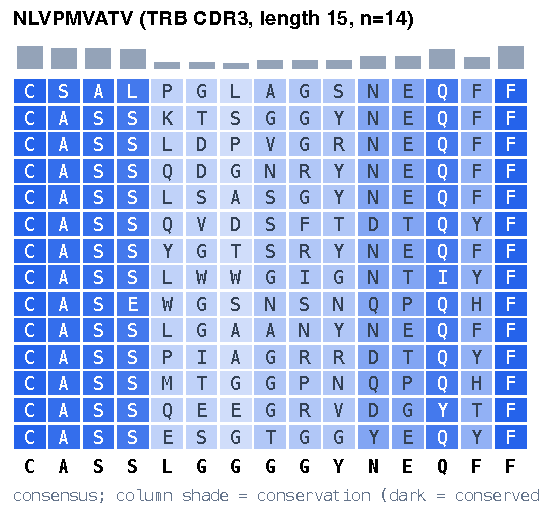
\includegraphics[width=0.66\linewidth]{aln/NLVPMVATV_msa.pdf}
  \caption{NLV (CMV pp65, A\textsuperscript{*}02) TRB CDR3 block; same conservation pattern.}
  \label{fig:nlv}
\end{figure}

\section{Limitations and roadmap}
The NDN matrix is estimated from a limited set of same-antigen single-substitution pairs and, at narrow
scope, matches rather than beats BLOSUM62; the region-aware V/J germline$+$trimming model (in progress)
and per-position weighting are expected to add discrimination, as is a per-chain treatment (TRA vs TRB)
and a V-gene similarity term (grouping V genes by CDR1/CDR2/CDR2.5 distance). The control's V--J usage
must match the query repertoire's, or the null is mis-specified; whether to renormalize V--J usage
(at the risk of erasing genuine V-gene bias) is an open question evaluated on held-out epitopes. These
extensions, and the full benchmark against existing tools, are the subject of ongoing work.

\bibliographystyle{plain}
\bibliography{refs}
\end{document}
